\documentclass[a4paper,14pt,russian,nocolumnsxix,nocolumnxxxii,nocolumnxxxi,hpadding=10mm]{eskdtext}

\usepackage{cmap}
\usepackage[T2A]{fontenc}
\usepackage[utf8x]{inputenc}
\usepackage[russian]{babel}
\usepackage{lastpage}
\usepackage{graphicx}

\renewcommand{\theenumi}{\arabic{enumi}} % Меняем везде перечисления на цифра.цифра
\renewcommand{\labelenumi}{\arabic{enumi}} % Меняем везде перечисления на цифра.цифра
\renewcommand{\theenumii}{.\arabic{enumii}} % Меняем везде перечисления на цифра.цифра
\renewcommand{\labelenumii}{\arabic{enumi}.\arabic{enumii}.} % Меняем везде перечисления на цифра.цифра
\renewcommand{\theenumiii}{.\arabic{enumiii}} % Меняем везде перечисления на цифра.цифра
\renewcommand{\labelenumiii}{\arabic{enumi}.\arabic{enumii}.\arabic{enumiii}.} % Меняем везде перечисления на цифра.цифра

\newcommand{\nocontentsline}[3]{}
\newcommand{\tocless}[2]{\bgroup\let\addcontentsline=\nocontentsline#1{#2}\egroup}

% Font settings
\linespread{1.3} % 1.5
\renewcommand{\rmdefault}{ftm} % Times new roman
\frenchspacing
%\ESKDsectStyle{section}{\normalsize} % Заголовки глав обычным шрифтом
%\ESKDsectStyle{subsection}{\normalsize} % Заголовки разделов обычным шрифтом
%\ESKDsectStyle{subsubsection}{\normalsize} % Заголовки подразделов обычным шрифтом

% defined macroses

\newcommand{\ksPersonField}[3]{
  \begin{minipage}[t]{0.40\textwidth}
    \begin{flushleft}
      #1 \\ #2 \\
      \hrulefill \hspace{0.1cm} #3 \\
      << \rule{1cm}{0.5pt} >> \hrulefill \hspace{0.1cm} \ESKDtheYear
    \end{flushleft}
  \end{minipage}
}

% styles

\renewcommand{\ESKDtitleFontI}{\ESKDfontIV}
\renewcommand{\ESKDtitleFontII}{\ESKDfontIV}
\renewcommand{\ESKDtitleFontIII}{\ESKDfontIV}
\renewcommand{\ESKDtitleFontIV}{\ESKDfontIV}
\renewcommand{\ESKDtitleFontV}{\ESKDfontIV}
\renewcommand{\ESKDtitleFontVI}{\ESKDfontIV}
\renewcommand{\ESKDtitleFontVII}{\ESKDfontIV}
\renewcommand{\ESKDtitleFontVIII}{\ESKDfontIV}
\renewcommand{\ESKDtitleFontIX}{\ESKDfontIV}
\renewcommand{\ESKDtitleFontX}{\ESKDfontIV}
\renewcommand{\baselinestretch}{1}

% data

\ESKDdepartment{ Министерство образования и науки Российской Федерации }
\ESKDcompany{
  Федеральное государственное бюджетное образовательное учреждение
  высшего профессионального образования \\
  <<Южно-Уральский государственный университет>> \\
  (национальный исследовательский университет) \\
  Факультет <<Приборостроительный>> \\
  Кафедра <<Электронные вычислительные машины>>
}

\ESKDauthor{М.А. Костюченко}
\ESKDchecker{}
\ESKDnormContr{}
\ESKDapprovedBy{К.А. Домбровский}
\newcommand{\ksSciDirector}{И.Л. Кафтанников}
\ESKDdate{2014/06/05}
\ESKDsignature{ЮУРГУ--ШИФР}
\ESKDletter{}{}{} % Литеры
\ESKDtitleDesignedBy{Автор работы, \\ студент группы ПС-427}{\ESKDtheAuthor} % Подпись и дата под заголовком документа

\ESKDdocName{Алгоритмизация визуальных представлений}
\renewcommand{\ESKDtheTitleFieldVI}{
  ПОЯСНИТЕЛЬНАЯ ЗАПИСКА \\
  К ВЫПУСКНОЙ КВАЛИФИКАЦИОННОЙ РАБОТЕ \\
  \ESKDtheSignature
}
 
\renewcommand{\ESKDtheTitleFieldII}{ 
  \ksPersonField{РАБОТА ПРОВЕРЕНА}{Рецензент}{}
  \hfill
  \ksPersonField{ДОПУСТИТЬ К ЗАЩИТЕ}{Заведующий кафедрой}{\ESKDtheApprovedBy}
}

\renewcommand{\ESKDtheTitleFieldVII}{
  \vspace{1.5cm}
  \hfill
  \ksPersonField{Руководитель проекта}{доцент каф. <<Электронные вычислительные машины>>}{\ksSciDirector}
}

\renewcommand{\ESKDtheTitleFieldVIII}{
  \hfill
  \ksPersonField{Автор работы}{студент группы ПС-427}{\ESKDtheAuthor} \\
  \vspace{2cm}
  \hfill
  \ksPersonField{Нормоконтролер}{}{}
}
 
\renewcommand{\ESKDtheTitleFieldX}{Челябинск \ESKDtheYear}


\begin{document}
  %\maketitle
  %\newpage
\section*{Аннотация}

\hfill
\begin{minipage}[t]{0.62\textwidth}
  \ESKDtheAuthor \space \ESKDtheDocName -- Челябинск ЮУрГУ, ПС, 2013. -- \ESKDtotal{page} с., 10~ил., библиогр. список~--~\ESKDtotal{bibitem}
\end{minipage} \\
\\

В данной работе рассмотрена разработка инструмента для создания визуальных
представлений, требующих параллельных вычислений на большом объеме данных, 
в веб-приложениях.

Целью дипломной работы явилось разработка программного инструмента для эффективного
создания визуальных представлений в веб-приложениях. Рассмотренные типы
визуализаций требуют особого подхода к вычислениям, так как отображают
взаимодействие большого количества частиц (от десяти тысяч) в реальном времени.
Подобный подход к вычислениям может быть использован для симуляции природных явлений 
и вычислении операций на большом количестве данных. Для достижения цели были поставлены
задачи: изучить способы визуализации данных в веб-приложениях с целью поиска эффективного
способа отображения, создание инструмента для визуализации и реализация демонстрационного 
примера для тестирования производительности.

Ожидаемые результаты:

\begin{itemize}
  \item эффективный способ визуализации сложных процессов в \\веб-приложениях;
  \item уменьшение времени на разработку подобных визуальных представлений.
\end{itemize}

Область применения -- обучающие сервисы, научные статьи и экспертные системы.

  \newpage
\section*{Введение}

%Проблема: есть некоторый описанный процесс . Задача сделать интерактивную визуализацию большого количества взаимодействующих объектов.
%Критерии: интерактивность -> реал-тайм, должно выполняться в браузере.
%Вопрос как выполнить это максимально рационально.
%Решение: Реализация основных алгоритмов, которые могут понадобиться при создании визуализации.
%Пример использования: визуализация пользовательских данных различных для каждого пользователя. При создании учебных курсов.  Создание визуализаций в экспертных системах. Кластеризация поисковой выдачи в ГИС.

%Графическое представление заметно способствует усваиванию информации.
%Современные компьютерные технологии помогают разрабатывать интерактивные и 
%наглядные изображения информации. Интерактивная визуализация информация -- подход
%к обработке информации в информационных системах, которая превращается в непрерывный 
%процесс взаимодействия с информацией через визуальное отображение.
%Приложения визуализации информации возникают в таких областях, как информационные
%системы и программное обеспечение, биологические науки, искусственный интеллект и 
%анализ пользовательских данных.

Визуальное представление информации -- это интерпретация числовой и текстовой
информации в виде графиков, структурных схем, таблиц, карт и т.д.
.... еще какая-нибудь хуита про интерактивную визуализацию.

Несмотря на развитие современных подходов к интерактивному отображению, задача
визуализации систем, требующих оперативного взаимодействие большого количества
объектов, все еще остается не тривиальной. Критериями эффективности решения
являются качество и доступность итоговой визуализации, а также время, необходимое
для ее создания.

Развитие параллельных вычислений с использованием графических процессоров сделало 
возможным визуализацию сложных интерактивных представлений информации. 

Веб приложения являются удачным решением быстрого донесения информации до большого
количества пользователей. Поддержка браузерами новых стандартов, таких как HTML5 и WebGL,  
позволила использовать преимущества вычислительных мощностей GPU в веб-приложениях.

Цель данной работы: поиск метода для эффективного создания визуальных представлений 
в веб-приложениях. Создания инструмента для интерактивного отображения и разработки
демонстрационного примера. В качестве демонстрации использования данного решения реализована 
визуализация вычислительного метода для симуляции жидкостей и газов -- гидродинамика 
сглаженных частиц.

%Легче воспринимать информацию с интерактивными примерами.
%Стоит задача как визуализировать процессы где требуется много вычислений.
%Современные компьютерная графика и постоянное развитие.
%Современные веб-технологии, кросс-платформенность и прочие плюхи веба.
%Использование webgl как инструмента для вычисления и визуализации.

 % 1 -> 2
  \newpage
\section{ОБЗОР АНАЛОГОВ}

\subsection{Стандарты}

Помимо используемого в работе WebGL так же разрабатывается стандарт WebCL, который описывает 
javascript-интерфейс стандарта OpenCL, т.е. API и расширения языка Си для организации
кросс-платформенных параллельных вычислений. Версия WebCL 1.0 была выпущена 19 марта 2014 года \cite{webcl10}.
Основным недостатком данного стандарта является отсутствие поддержки большинством браузеров.

\subsection{Библиотеки}
Существует множество библиотек для визуализации в веб-приложениях. Функционал который они реализуют:
\begin{itemize}
  \item Изображение графиков
  \item Построение графов
  \item Визуализация 3-х мерных объектов
\end{itemize}

Примеры:
\begin{itemize}
  \item Three.js -- кроссбраузерная библиотека JavaScript для создания анимированной 3D графики.
    Предоставляет полный доступ ко всем WebGL шейдерам. Может совместно использоваться с элементом
    HTML5 CANVAS, SVG или WebGL. Реализована работа с кадровыми буферами (framebuffer).

  \item Highcharts -- библиотека для построения интерактивных графиков в веб-проектах. Предоставляет
    богатый API для создания наглядных визуальных представлений.

  \item D3.js -- библиотека для визуализации данных. Позволяет изобразить данные в HTML формате. 
    К примеру, построить таблицу из массива чисел.
    
  \item Cytoscape.js -- библиотека для анализа и визуализации. Позволяет автоматически 
    строить различные типы графов.
\end{itemize}

Недостаток данных решений: они реализуют исключительно визуализацию данных, таким образом реализация
алгоритмов ложится на плечи программистов. Отсюда следует что они только частично решают поставленную
задачу.
 % 2
  \newpage
\section{ОСОБЕННОСТИ ВЫЧИСЛЕНИЙ НА GPU}

\subsection{Преимущества перед решением на ЦП}

Задача интерактивной визуализации состоит не только в изображении, но и в просчете данных.
В случае с большим количеством оперативно взаимодействующих между собой объектов, вычисление
на графическом процессоре может значительно увеличить производительность за счет параллельности,
заложенной в архитектуру графической карты. В этом случае данные о каждой из частиц могут быть
представлены либо как вершинные, либо храниться в кадровых буферах.

После обработки данных, информация о каждом объекте уже будет храниться в памяти графической карты.
Это значит что для визуализации достаточно вывести содержимое на экран.

\subsection{Графический конвейер}

Графический конвейер -- основной компонент компьютерной графики. Задача конвейера преобразовать
данные трехмерные объекты, источники света, виртуальную камеру и шейдерные преобразования в 
двумерное изображение.

Первые версии конвейеров работали с жесткой логикой (Fixed-Function Pipeline) \cite{raytracing02}.
Программисты не имели особого контроля над процедурой визуализации, потому что большинство
операций было встроено в аппаратное обеспечение и их невозможно было изменить программно.

Современные графические процессоры предоставляют так называемый программируемый графический
конвейер, который позволяет программистам писать специальные программы (шейдеры), которые
описывают поведение конвейера. При правильном использовании, шейдеры могут быть весьма эффективным
инструментом для создания различных эффектов. GPU состоят из сотен поточных процессоров и следуют
принципу параллельных вычислений SIMD (Single Instruction, Multiple Data) \cite{gpu}. Таким образом
параллелизм осуществляется на уровне данных, когда одна и та же операция выполняется
на множестве данных.

Сам конвейер состоит из следующих частей \cite{hgpuw}:

\begin{enumerate}
  \item Массивы данных из центрального процессора загружаются на графический в вершинный буфер
    (vertex buffer object).

  \item Проходят через вершинный шейдер (vertex shader), в котором подвергаются обработке 
    непосредственно сами элементы массива. Обычно на данном этапе идут преобразования 
    координат объектов для афинных преобразований и создания перспективы. Так же 
    могут быть преобразования цвета и координат текстур, но создание новых вершин 
    (элементов) не возможно.

  \item Следующий шаг это геометрический шейдер. Данный тип программ не поддерживается
    стандартом WebGL. Однако реализован в новых графических процессорах. В отличие 
    от вершинного, геометрический шейдер может обрабатывать одновременно целые примитивы 
    (отрезок, треугольник и т.д.). Кроме того, есть возможность генерировать примитивы 
    ``на лету'' не задействуя при этом центральный процессор.

  \item Затем полученные вершины попадают на сборку (clipping). На этом этапе образуются
    примитивы. Вершины, которые выходят из радиуса видимости, отбрасываются.

  \item Растеризация. Трехмерные примитивы преобразуются в двухмерные фигуры. Каждая фигура
    разбивается на фрагменты размером с пиксель.

  \item Фрагментный (или пиксельный) шейдер. На этом этапе задается цвет каждого из фрагментов.
    Самый простой фрагментный шейдер формирует один пиксель в виде цвета. Более сложные могут 
    выводить до нескольких цветов одновременно. Данные программы имеют информацию о положении 
    точки на экране, текстуре и других данных, передаваемых между шейдерами.

  \item Полученное изображение записывается в буфер кадра и выводится на экран (если необходимо).
\end{enumerate}

Данные шаги и передаваемые между ними данные изображены на рисунке \ref{fig:gpu_pipeline}.

\begin{figure}
\begin{center}
  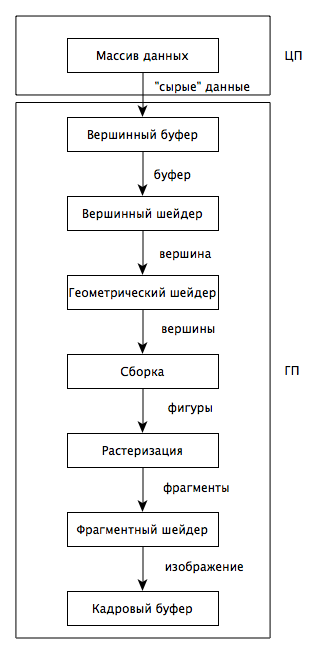
\includegraphics[scale=1.0]{Figures/gpu_pipeline}
\end{center}
\caption{Программируемый графический конвейер}
\label{fig:gpu_pipeline}
\end{figure}


\subsection{Язык шейдеров}

WebGL основан на стандарте OpenGL ES 2.0 \cite{khr11}, который поддерживает только программируемый графический
конвейер. Язык программирования, используемый для написания шейдеров, называется GLSL (OpenGL
Shading Language).

Поддерживаемые в данном стандарте типы шейдеров:

\begin{enumerate}
  \item Вершинные шейдеры. На входе: вершина фигуры. На выходе: преобразованное положение
    вершины. Результат вычислений записывается в специальную переменную gl\textunderscore{}Position.
  \item Фрагментные шейдеры. На входе: координаты на экране и данные, переданные из вершинного 
    шейдера. На выходе: цвет пикселя. Результат записывается в переменную gl\textunderscore{}FragColor.
\end{enumerate}

Когда вершинные и фрагментные шейдеры скомпилированы, они связываются в шейдерную программу.
В каждой программе может содержаться только один вершинный шейдер.

Доступность данных передаваемых внутри программ зависят от того, где они были инициализированы
и строго определяется какие операции могут на них выполнятся. В спецификации GLSL ES 1.0 
существует пять различных модификаторов типов:

\begin{itemize}
  \item Локальные переменные (по умолчанию без ключевого слова)
  \item Константы (ключевое слово const). Значения данного типа формируются во время компиляции и их не
    разрешено изменять при работе программы.
  \item Аттрибуты (ключевое слово attribute). Загружаются на видеокарту из центрального процессора во время передачи массива данных. Видимы в 
    вершинных шейдерах. Значения данного типа так же доступны в режиме только на чтение.
  \item Одинаковые для всех шейдеров (ключевое слово uniform). Передаются с ЦП во время 
    использования программы. Доступны как в вершинных, так и в фрагментных.
  \item Последний модификатор формирует связь между вершинным и фрагментным шейдером. Первый
    формирует какое-то значение для каждой вершины и передает его в вершинную программу.
    Ключевое слово varying.
\end{itemize}

\subsection{Кадровые буферы}

Кадровым буфером называется область памяти для кратковременного хранения данных перед отправкой
на устройство вывода. Данный буфер содержит полную информацию о цветах (значениях) кадра.

Значения кадрового буфера формируется на выходе фрагментного шейдера. Это значит что их можно 
использовать как промежуточное хранилище данных при выполнении алгоритмов. Этап формирования 
конечного изображения через множество программ называются проходом (pass). Содержимое буферов 
можно считывать по известным координатам. Получаемые данные носят название тексел (текстурный 
пиксел). В данном подходе данные остаются непосредственно на видеокарте. Уходит необходимость
постоянно передавать данные на ЦП и обратно, что значительно увеличивает производительность.

Тип данных кадровых буферов определяется стандартом. Выход фрагментных шейдеров представлен в 
GLSL как четырехмерный вектор типа float (числа с плавающей точкой). Передача в другую программу
осуществляется через текстурные блоки. В спецификации WebGL по-умолчанию при связке текстуры
и кадрого буфера доступен только формат byte (неотрицательное число от 0 до 255) \cite{khr11}. 
Это значит что при вычислениях могут быть значительные потери при дискретизации данных. При помощи
расширения OES\textunderscore{}texture\textunderscore{}float можно включить поддержку передачи 
данных типа float.
 % 4 -> 5?? (pictures)
  \newpage
\section{Реализация}

\subsection{Технологии и библиотеки}

Как говорилось ранее, проект реализован под веб-платформу. Для разработки используются следующие технологии:

\begin{itemize}
  \item HTML5 -- язык разметки, используемый для построения структуры и представления веб-страниц. 
    Это пятая версия языка, которая добавляет поддержку тэга \textless{}canvas\textgreater{}, 
    который позволяет скриптовому попиксельному отображению изображений через различные контексты. 
    На момент написания работы, доступно два основных контекста: 2d и webgl.

    2D был первым реализованным типом контекста. Он реализован как абстрактный автомат (схоже 
    с OpenGL) и может быть использован для высокопроизводительной визуализации двухмерных объектов, 
    таких как линии, прямоугольники, кривые, bitmap-изображения и т.д.

    Следующий тип контекста позволил разработчикам создавать высокопроизводительные 3D изображения 
    без использования сторонних плагинов и расширений. Это значит что пользователям не требуется 
    устанавливать дополнительное ПО (например, Adobe Flash Player или Java VM) для просмотра.

  \item Javascript -- динамичный язык программирования. Используется для взаимодействия с 
    пользователями, контроля браузером и асинхронной загрузки ресурсов.

  \item Coffeescript -- язык программирования, который транслируется в javascript. Добавляет 
    синтаксический сахар для повышения краткости и читаемости кода. Например, классы 
    (из объектно-ориентированного программирования), которые имеют четкую и понятную структуру.

  \item WebGL -- спецификация интерфейса для создания динамичных 2D и 3D сцен без использования 
    сторонних плагинов. Создан и поддерживается организацией Khronos Group, на данный момент, 
    разрабатывающей спецификацию OpenGL. WebGL служит связкой между высокоуровневым языком 
    JavaScript и низкоуровневыми операциями на графических процессорах.

  \item GLSL (OpenGL Shading Language) -- язык высокого уровня для программирования шейдеров. 
    Основным преимуществом GLSL является переносимость между платформами и ОС. Т.е. алгоритмы, 
    описанные в рамках данной работы, могут быть перенесены на другие платформы без изменения 
    кода программы.
\end{itemize}

Для упрощения разработки используется Zepto.js. Zepto.js -- библиотека для расширения функционала 
javascript. В частности реализует работу с AJAX запросами, которые используются для загрузки 
ресурсов. Является минималистичным аналогом jQuery, который также может являться альтернативой.

Основным преимуществом данного подхода к реализации является платформонезвисиммость и быстрота разработки.

\subsection{Общая архитектура}
\subsection{Описание алгоритмов}
\subsubsection{Сортировка}
\subsubsection{Поиск ближайших}
\subsubsection{Кластеризация}
\subsubsection{SPH}
 % 2 -> 5
  \newpage

  \section{Техническое задание} % 2
  %\section{Сравнение аналогов}
  %\section{Особенности вычисления на GPU}
  \section{Тестирование производительности} % 1
  \section{Примеры использования} % 3
  \subsection{Учебные курсы}
  \subsection{Визуальные представления в экспертных системах}
  \subsection{Кластеризация поисковой выдачи в ГИС}
  \section{Руководство по использованию} % 2
  \section{Заключение} % 2
  \newpage
  \tableofcontents 
\end{document}
